\section{Structural Diagnosis: Where Does Output Geometry Live?}
\label{sec:diagnosis}

Before designing an output-side preconditioner, we ask an empirical question across unpreconditioned, input-whitened, and two-sided preconditioned training: \emph{what is the actual covariance and temporal structure of every input activation and output cotangent in a Transformer, and does active preconditioning alter that geometry?}
Auditing three matched trajectories---\mname{Muon}, \mname{MuonT}, and \mname{WT-MLP-Lag}---separates intrinsic architectural invariants of pre-RMSNorm SwiGLU Transformers from optimizer-induced adaptation.

\subsection{Preliminaries and Three-Trajectory Moment Audit}
\label{sec:diagnosis_setup}

Consider a 2D linear projection $y = W x$ with weight $W_t \in \R^{m \times n}$ at step $t$ (rows index output coordinates $m$; columns index input coordinates $n$).
In a Llama-style pre-RMSNorm Transformer block with hidden width $\dm$ and SwiGLU expansion width $\dff = 4\dm$, each layer $\ell \in \{1,\dots,L\}$ contains seven 2D projections:
four square attention matrices $W_q, W_k, W_v, W_o \in \R^{\dm \times \dm}$, two tall MLP expansion matrices $W_{\mathrm{gate}}, W_{\mathrm{up}} \in \R^{\dff \times \dm}$, and one wide MLP contraction matrix $W_{\mathrm{down}} \in \R^{\dm \times \dff}$.

\paragraph{Input vs.\ output second moments.}
During forward and backward propagation over $N_t$ sampled token positions pooled globally across ranks and microbatches ($286$ positions per $4{,}096$-token sequence, $N_t = 36{,}608$ per $0.5\text{M}$-token batch), each projection observes activations $x_{p,t,j} \in \R^{n_p}$ and unaveraged summed-loss output cotangents $\delta_{p,t,j} = \partial \sum \ell / \partial y_{p,t,j} \in \R^{m_p}$, yielding exponential moving averages (EMAs):
\begin{equation}
  C_{g(p),t} = \beta C_{g(p),t-1} + \frac{1-\beta}{N_t}\sum_{j=1}^{N_t} x_{p,t,j} x_{p,t,j}^{\Tr},
  \qquad
  B_{p,t} = \beta B_{p,t-1} + \frac{1-\beta}{N_t}\sum_{j=1}^{N_t} \delta_{p,t,j} \delta_{p,t,j}^{\Tr},
  \label{eq:moments}
\end{equation}
with $\beta = 0.938$ (effective averaging horizon $(1-\beta)^{-1} \approx 16.1$ updates).
Crucially, sharing differs between the two sides: because $W_q, W_k, W_v$ consume identical post-RMSNorm activations and $W_{\mathrm{gate}}, W_{\mathrm{up}}$ consume identical MLP post-RMSNorm activations, there are only 4 input moments per layer (\texttt{in:attn}, \texttt{in:o}, \texttt{in:mlp} at width $\dm$; \texttt{in:down} at width $\dff$).
On the output side, however, every projection receives a distinct backpropagated cotangent---even \texttt{out:o} and \texttt{out:down} write to sequential residual nodes separated by the MLP---requiring 7 separate output moments per layer ($5$ at width $\dm$ and $2$ at width $\dff$, or $224$ matrices across $L=32$ layers).

\paragraph{Trace-normalized inverse roots, three trajectories, and three diagnostic metrics.}
Following \mname{MuonT}~\citep{mohamadi2026toner}, any positive-trace symmetric moment $F \in \R^{d \times d}$ is trace-normalized and damped via
\begin{equation}
  A_d(F) = \frac{d\,F}{\tr(F)} + \epsilon I_d, \qquad \epsilon = 10^{-3},
  \label{eq:trace_norm}
\end{equation}
so that an isotropic moment satisfies $A_d(\alpha I_d) = (1+\epsilon)I_d$ and any constant positive cotangent scaling cancels identically.
From $A_d(F)$, \mname{MuonT} forms split inner and unit-RMS outer inverse roots $\mathsf{In}_d(F) = A_d(F)^{-1/2}$ and $\mathsf{Out}_d(F) = \sqrt{d}\,A_d(F)^{-1/8} / \|A_d(F)^{-1/8}\|_F$.

To audit all $11 \times 32 = 352$ full $d \times d$ FP32 moments at matched \texttt{130M} ($\dm=512, \dff=2048$, \texttt{seed 0}, $0.5\text{M}$ batch), we examine three trajectories:
(i) \mname{Muon} ($\eta=0.016$), via an exact $500$-step passive moment replay from the saved step-$2{,}000$ checkpoint through steps $2{,}250$ and $2{,}500$ ($0.0$ loss and weight divergence; $\beta^{250} = 1.1\times 10^{-7}$ and $\beta^{500} = 1.3\times 10^{-14}$ residual initialization weight);
(ii) \mname{MuonT} ($\eta=0.02263$, recorded via \mname{Null-Dense} across $10$ checkpoints over all $5{,}120$ steps while applying $L=\hat{L}=I$); and
(iii) \mname{WT-MLP-Lag} ($\eta=0.02263$, abbreviated \mname{WT} in \Cref{tab:diagnosis}), via a $500$-step \texttt{fast\_lag} replay through steps $2{,}250$ and $2{,}500$ that records all nine active dense groups alongside passive $2{,}048\times 2{,}048$ \texttt{out:gate,up} moments (matching active 1D diagonal accumulators to $\le 4.0\times 10^{-5}$ relative $\ell_2$ error across all 8 ranks; see \Cref{app:appendix_mech}).
On $\tilde{A} = d\,F/\tr(F)$ (unit mean diagonal $\frac{1}{d}\tr(\tilde{A}) = 1$), we evaluate:
\begin{enumerate}[leftmargin=1.6em, itemsep=2pt, topsep=3pt]
  \item \textbf{Pythagorean diagonal anisotropy share:}
  Because $\|\tilde{A} - I_d\|_F^2 = \|\diag(\tilde{A}) - \mathbf{1}\|_2^2 + \|\tilde{A} - \Diag(\tilde{A})\|_F^2$ holds to machine precision,
  \begin{equation}
    \mathrm{DiagAniso}(F) \triangleq \frac{\|\diag(\tilde{A}) - \mathbf{1}\|_2^2}{\|\tilde{A} - I_d\|_F^2} \in [0, 1]
    \label{eq:diag_aniso}
  \end{equation}
  measures the exact fraction of total departure-from-isotropy variance carried by per-coordinate scale differences rather than off-diagonal cross-coordinate correlations (quantified alongside the off-diagonal correlation RMS $\rho_{\mathrm{rms}} = \bigl[\frac{1}{d(d-1)}\sum_{i\neq j} F_{ij}^2/(F_{ii}F_{jj})\bigr]^{1/2}$).
  \item \textbf{Diagonal inverse-root explained variance:}
  Comparing the dense inner root $L = A_d(F)^{-1/2}$ to its elementwise diagonal counterpart $L_{\diag} = \Diag(\tilde{A} + \epsilon I_d)^{-1/2}$,
  \begin{equation}
    R^2(A_d^{-1/2}) \triangleq 1 - \frac{\|L - L_{\diag}\|_F^2}{\|L - I_d\|_F^2}
    \label{eq:r2_root}
  \end{equation}
  measures how much of the dense whitening operator's nontrivial action is captured by O($d$) coordinate scaling alone.
  \item \textbf{Subspace Grassmann drift:}
  Letting $V_{k,t} \in \R^{d \times k}$ denote the top-$k$ eigenvectors of $F_t$, $\mathrm{Drift}_{16}(t) \triangleq 1 - \frac{1}{16}\|V_{16,t}^{\Tr}V_{16,t-250}\|_F^2 = \frac{1}{32}\|V_{16,t}V_{16,t}^{\Tr} - V_{16,t-250}V_{16,t-250}^{\Tr}\|_F^2 \in [0,1]$ measures how rapidly the dominant 16-dimensional eigenspace rotates over $250$ updates.
\end{enumerate}

\begin{table}[t]
  \centering
  \caption{\textbf{Three-trajectory structural and temporal audit across all 11 Transformer second moments} (\texttt{130M}, $352$ FP32 EMA matrices across $L=32$ layers) comparing unpreconditioned \mname{Muon}, input-whitened \mname{MuonT}, and active two-sided \mname{WT-MLP-Lag} (\mname{WT}). Metric groups 1--5 report step-$2{,}500$ ($1.31\text{B}$-token) 32-layer medians; $\mathrm{Drift}_{16}$ reports the 32-layer mean over steps $2{,}250 \to 2{,}500$. Across all three trajectories, pre-SwiGLU expansion outputs (\texttt{out:gate}, \texttt{out:up}) hug the $0.0052$ sampling floor with $78\%\text{--}91\%$ diagonal anisotropy ($R^2 = 76\%\text{--}99\%$), whereas residual-stream outputs (\texttt{out:o}, \texttt{out:down}) remain $\ge 99\%$ rotational ($\mathrm{DiagAniso} = 0.8\%\text{--}1.0\%$).}
  \label{tab:diagnosis}
  \vspace{2pt}
  \footnotesize\setlength{\tabcolsep}{2.3pt}%
  \resizebox{\textwidth}{!}{%
  \begin{tabular}{@{}l@{\hspace{6pt}}r@{\hspace{9pt}}rrr@{\hspace{9pt}}rrr@{\hspace{9pt}}rrr@{\hspace{9pt}}rrr@{\hspace{9pt}}rrr@{\hspace{9pt}}rrr@{}}
    \toprule
    & & \multicolumn{3}{c@{\hspace{9pt}}}{$\mathrm{erank}/d$ (\%)} & \multicolumn{3}{c@{\hspace{9pt}}}{$\mathrm{CV}_{\diag}$} & \multicolumn{3}{c@{\hspace{9pt}}}{$\rho_{\mathrm{rms}}$} & \multicolumn{3}{c@{\hspace{9pt}}}{$\mathrm{DiagAniso}$ (\%)} & \multicolumn{3}{c@{\hspace{9pt}}}{$R^2(A_d^{-1/2})$ (\%)} & \multicolumn{3}{c@{}}{$\mathrm{Drift}_{16}$} \\
    \cmidrule(r{9pt}){3-5}\cmidrule(r{9pt}){6-8}\cmidrule(r{9pt}){9-11}\cmidrule(r{9pt}){12-14}\cmidrule(r{9pt}){15-17}\cmidrule{18-20}
    Moment Group & $d$ & \multicolumn{1}{c}{\tiny\mname{Muon}} & \multicolumn{1}{c}{\tiny\mname{MuonT}} & \multicolumn{1}{c@{\hspace{9pt}}}{\tiny\mname{WT}} & \multicolumn{1}{c}{\tiny\mname{Muon}} & \multicolumn{1}{c}{\tiny\mname{MuonT}} & \multicolumn{1}{c@{\hspace{9pt}}}{\tiny\mname{WT}} & \multicolumn{1}{c}{\tiny\mname{Muon}} & \multicolumn{1}{c}{\tiny\mname{MuonT}} & \multicolumn{1}{c@{\hspace{9pt}}}{\tiny\mname{WT}} & \multicolumn{1}{c}{\tiny\mname{Muon}} & \multicolumn{1}{c}{\tiny\mname{MuonT}} & \multicolumn{1}{c@{\hspace{9pt}}}{\tiny\mname{WT}} & \multicolumn{1}{c}{\tiny\mname{Muon}} & \multicolumn{1}{c}{\tiny\mname{MuonT}} & \multicolumn{1}{c@{\hspace{9pt}}}{\tiny\mname{WT}} & \multicolumn{1}{c}{\tiny\mname{Muon}} & \multicolumn{1}{c}{\tiny\mname{MuonT}} & \multicolumn{1}{c@{}}{\tiny\mname{WT}} \\
    \midrule
    \multicolumn{20}{@{}l}{\emph{Right-input second moments $C_t = \E[x x^{\Tr}]$ (4 per layer, 128 total)}} \\
    \texttt{in:attn} ($q,k,v$)       & 512  & $30.0$ & $17.9$ & $18.0$ & $0.63$ & $0.84$ & $0.76$ & $0.1465$ & $0.2031$ & $0.2066$ & $1.4$ & $1.0$ & $0.8$ & $8.2$ & $10.6$ & $10.1$ & $0.041$ & $0.021$ & $0.023$ \\
    \texttt{in:o}                    & 512  & $37.9$ & $20.8$ & $23.4$ & $0.77$ & $0.75$ & $0.77$ & $0.0968$ & $0.2120$ & $0.2001$ & $9.8$ & $1.8$ & $1.8$ & $30.1$ & $22.5$ & $26.5$ & $0.107$ & $0.094$ & $0.108$ \\
    \texttt{in:mlp} ($\text{gate,up}$) & 512 & $33.8$ & $21.6$ & $19.5$ & $0.48$ & $0.64$ & $0.62$ & $0.1410$ & $0.1959$ & $0.2024$ & $1.0$ & $0.8$ & $0.7$ & $4.9$ & $6.0$ & $6.7$ & $0.046$ & $0.021$ & $0.025$ \\
    \texttt{in:down} (post-SwiGLU)   & 2048 & $67.1$ & $29.1$ & $35.6$ & $0.71$ & $2.92$ & $2.33$ & $0.0283$ & $0.0346$ & $0.0359$ & $20.3$ & $43.4$ & $34.7$ & $91.3$ & $79.4$ & $78.7$ & $0.186$ & $0.106$ & $0.087$ \\
    \addlinespace[2.5pt]
    \multicolumn{20}{@{}l}{\emph{Left-cotangent second moments $B_t = \E[\delta \delta^{\Tr}]$ (7 per layer, 224 total)}} \\
    \texttt{out:q}                   & 512  & $38.5$ & $38.5$ & $29.3$ & $1.04$ & $0.97$ & $1.14$ & $0.0615$ & $0.0641$ & $0.0732$ & $16.4$ & $18.0$ & $13.3$ & $64.8$ & $62.4$ & $66.0$ & $0.150$ & $0.140$ & $0.110$ \\
    \texttt{out:k}                   & 512  & $24.4$ & $23.7$ & $13.0$ & $1.45$ & $1.50$ & $1.87$ & $0.0746$ & $0.0774$ & $0.0779$ & $15.5$ & $14.4$ & $14.7$ & $77.6$ & $71.8$ & $78.6$ & $0.178$ & $0.165$ & $0.147$ \\
    \texttt{out:v}                   & 512  & $47.0$ & $50.4$ & $41.5$ & $0.63$ & $0.58$ & $0.57$ & $0.0600$ & $0.0560$ & $0.0749$ & $11.5$ & $12.2$ & $6.8$ & $38.6$ & $31.2$ & $19.9$ & $0.664$ & $0.662$ & $0.586$ \\
    \textcolor{colWT}{\textbf{\texttt{out:o} (residual)}}    & \textcolor{colWT}{\textbf{512}} & $83.3$ & $85.3$ & $78.2$ & $0.09$ & $0.06$ & $0.10$ & $0.0307$ & $0.0301$ & $0.0393$ & \textcolor{colWT}{$\mathbf{1.0}$} & \textcolor{colWT}{$\mathbf{0.8}$} & \textcolor{colWT}{$\mathbf{0.8}$} & \textcolor{colWT}{$\mathbf{3.6}$} & \textcolor{colWT}{$\mathbf{1.2}$} & \textcolor{colWT}{$\mathbf{2.3}$} & $0.164$ & $0.134$ & $0.103$ \\
    \textcolor{colWT}{\textbf{\texttt{out:down} (residual)}} & \textcolor{colWT}{\textbf{512}} & $84.3$ & $84.6$ & $77.9$ & $0.08$ & $0.07$ & $0.09$ & $0.0315$ & $0.0312$ & $0.0403$ & \textcolor{colWT}{$\mathbf{0.9}$} & \textcolor{colWT}{$\mathbf{0.8}$} & \textcolor{colWT}{$\mathbf{0.8}$} & \textcolor{colWT}{$\mathbf{2.3}$} & \textcolor{colWT}{$\mathbf{1.2}$} & \textcolor{colWT}{$\mathbf{1.4}$} & $0.123$ & $0.107$ & $0.072$ \\
    \rowcolor{rowtint}
    \textcolor{colOD}{\textbf{\texttt{out:gate} (pre-SwiGLU)}} & \textcolor{colOD}{\textbf{2048}} & $88.2$ & $87.1$ & $72.8$ & $0.55$ & $0.59$ & $1.32$ & \textcolor{colOD}{$\mathbf{0.0055}$} & \textcolor{colOD}{$\mathbf{0.0051}$} & \textcolor{colOD}{$\mathbf{0.0048}$} & \textcolor{colOD}{$\mathbf{80.6}$} & \textcolor{colOD}{$\mathbf{82.0}$} & \textcolor{colOD}{$\mathbf{89.5}$} & \textcolor{colOD}{$\mathbf{98.8}$} & \textcolor{colOD}{$\mathbf{82.2}$} & \textcolor{colOD}{$\mathbf{94.9}$} & $0.292$ & $0.240$ & $0.159$ \\
    \rowcolor{rowtint}
    \textcolor{colOD}{\textbf{\texttt{out:up} (pre-SwiGLU)}}   & \textcolor{colOD}{\textbf{2048}} & $83.8$ & $82.5$ & $47.3$ & $0.68$ & $0.75$ & $2.83$ & \textcolor{colOD}{$\mathbf{0.0068}$} & \textcolor{colOD}{$\mathbf{0.0073}$} & \textcolor{colOD}{$\mathbf{0.0082}$} & \textcolor{colOD}{$\mathbf{77.9}$} & \textcolor{colOD}{$\mathbf{78.1}$} & \textcolor{colOD}{$\mathbf{90.8}$} & \textcolor{colOD}{$\mathbf{98.2}$} & \textcolor{colOD}{$\mathbf{75.9}$} & \textcolor{colOD}{$\mathbf{91.9}$} & $0.251$ & $0.215$ & $0.130$ \\
    \bottomrule
  \end{tabular}%
  }
\end{table}

\subsection{Finding 1: The Width-and-Role Dichotomy Across Output Moments}
\label{sec:dichotomy}

\Cref{tab:diagnosis} and \Cref{fig:structural_audit}a reveal that output cotangent moments partition sharply into three architectural regimes governed by projection width and nonlinearity placement---a dichotomy that holds across unpreconditioned \mname{Muon}, input-whitened \mname{MuonT}, and active two-sided \mname{WT-MLP-Lag} (as well as full dense \mname{DT-All}; \Cref{app:appendix_mech}):

\paragraph{1. Expanded pre-SwiGLU outputs (\texttt{out:gate}, \texttt{out:up}; $d = \dff$) are coordinate-dominated across all three optimizers.}
Because SwiGLU computes $z = \operatorname{SiLU}(y_{\mathrm{gate}}) \odot y_{\mathrm{up}}$ elementwise across the $\dff$ intermediate channels, backpropagating through the elementwise gate multiplies each coordinate by a weakly correlated gate factor, driving cross-channel correlations toward zero while compounding coordinate variance spread.
Across \mname{Muon} / \mname{MuonT} / \mname{WT-MLP-Lag}, \texttt{out:gate} and \texttt{out:up} concentrate $94.9\% / 94.9\% / 94.1\%$ and $91.9\% / 91.2\% / 92.4\%$ of their raw Frobenius energy and $80.6\% / 82.0\% / 89.5\%$ and $77.9\% / 78.1\% / 90.8\%$ of their centered anisotropy ($\mathrm{DiagAniso}$) on the diagonal, while their off-diagonal correlation RMS ($\rho_{\mathrm{rms}} = 0.0055 / 0.0051 / 0.0048$ and $0.0068 / 0.0073 / 0.0082$) sits directly at the finite-sample floor $1/\sqrt{N_t} = 0.0052$!
Consequently, an $O(\dff)$ diagonal inverse root explains $98.8\% / 82.2\% / 94.9\%$ and $98.2\% / 75.9\% / 91.9\%$ of dense $A_d(B)^{-1/2}$ across all 32 layers ($\cos(L, L_{\diag}) = 0.996\text{--}0.998$ on \texttt{gate} and $0.993\text{--}0.997$ on \texttt{up}): active inline diagonal normalization under \mname{WT-MLP-Lag} induces zero off-diagonal coupling while deepening per-neuron scale specialization ($\mathrm{CV}_{\diag}$ rising from $0.55 / 0.59$ to $1.32$ on \texttt{gate} and from $0.68 / 0.75$ to $2.83$ on \texttt{up}).

\paragraph{2. Residual-stream writers (\texttt{out:o}, \texttt{out:down}; $d = \dm$) are $\ge 99\%$ rotational on every trajectory.}
At the opposite extreme, projections writing directly into the shared residual stream exhibit uniform per-coordinate cotangent variance under every optimizer ($\mathrm{CV}_{\diag} = 0.09 / 0.06 / 0.10$ on \texttt{out:o} and $0.08 / 0.07 / 0.09$ on \texttt{out:down}).
As a result, $\mathrm{DiagAniso}$ collapses to $0.8\%\text{--}1.0\%$, and diagonal inverse roots capture only $1.2\%\text{--}3.6\%$ of $A_d(B)^{-1/2}$ ($R^2 \le 2.5\%$ across \mname{MuonT}'s entire 8-checkpoint trajectory)!
Yet $B_o$ and $B_{\mathrm{down}}$ are far from isotropic (mean top-to-mean eigenvalue ratios $42.4$ and $40.5$ on \mname{MuonT}), making any purely diagonal output preconditioner (\mname{OD-All}) nearly an identity map on $W_o$ and $W_{\mathrm{down}}$.

\paragraph{3. Attention internal outputs (\texttt{out:q,k,v}; $d = \dm$) and post-SwiGLU inputs (\texttt{in:down}; $d = \dff$) are mixed.}
Within attention, \texttt{out:q} and \texttt{out:k} combine head-level scale variation with rotary/attention-score coupling ($R^2 = 62.4\%\text{--}66.0\%$ and $71.8\%\text{--}78.6\%$), while \texttt{out:v} remains predominantly rotational ($\mathrm{DiagAniso} = 6.8\%\text{--}12.2\%, R^2 = 19.9\%\text{--}38.6\%$).
On the input side, RMSNormed \texttt{in:attn} and \texttt{in:mlp} are $98.6\%$--$99.3\%$ rotational across all three runs ($\mathrm{DiagAniso} = 0.7\%$--$1.4\%$; active input whitening sharpens \texttt{in:attn} $\mathrm{erank}/d$ from $30.0\%$ on \mname{Muon} to $17.9\% / 18.0\%$ on \mname{MuonT} / \mname{WT}), whereas post-SwiGLU \texttt{in:down} retains $79.7\%$, $56.6\%$, and $65.3\%$ off-diagonal moment anisotropy across \mname{Muon}, \mname{MuonT}, and \mname{WT-MLP-Lag} ($\rho_{\mathrm{rms}} = 0.0283 / 0.0346 / 0.0359$, $5.1\times$--$7.5\times$ above \texttt{out:gate}) alongside large coordinate skew ($R^2 = 91.3\% / 79.4\% / 78.7\%$).

\begin{figure}[t]
  \centering
  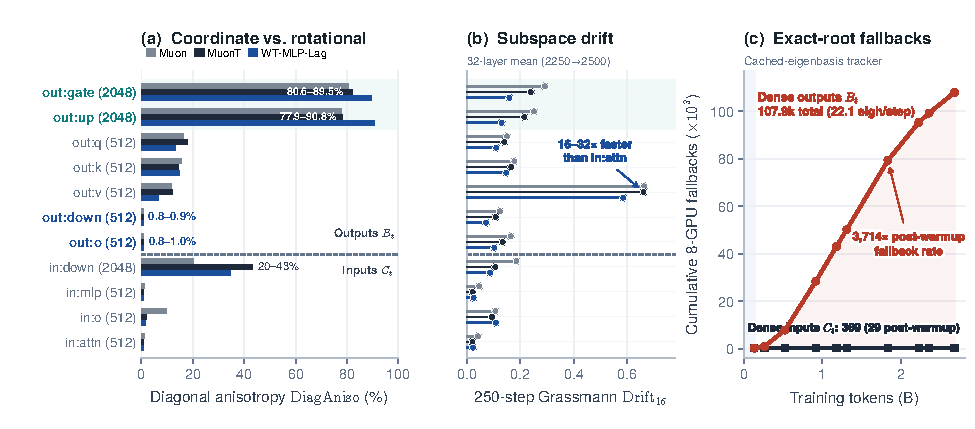
\includegraphics[width=\textwidth]{fig2_structural_audit.pdf}
  \caption{\textbf{Three-trajectory structural and temporal anatomy of the 11 Transformer second moments (\texttt{130M}).}
  \textbf{(a)} Pythagorean diagonal anisotropy share ($\mathrm{DiagAniso}$) across \mname{Muon}, \mname{MuonT}, and \mname{WT-MLP-Lag} consistently separates coordinate-dominated $\dff=2048$ MLP outputs (\texttt{out:gate} $80.6\%$--$89.5\%$, \texttt{out:up} $77.9\%$--$90.8\%$) from rotation-dominated $\dm=512$ residual outputs (\texttt{out:o, down} $0.8\%$--$1.0\%$) and inputs.
  \textbf{(b)} Backward cotangent top-16 eigenspaces drift an order of magnitude faster over 250 steps than RMSNormed forward activations across all three trajectories ($16\times$--$32\times$ faster on \texttt{out:v} vs.\ \texttt{in:attn}).
  \textbf{(c)} Rapid subspace drift causes Toner's cached-eigenbasis root solver on \mname{Null-Dense} (\mname{MuonT}) to trigger $107{,}911$ exact eigendecomposition fallbacks on dense outputs ($22.1/\text{step}$) vs.\ only $369$ ($29$ post-warmup) on inputs.}
  \label{fig:structural_audit}
\end{figure}

\subsection{Finding 2: Cubic Cost Concentration and Subspace Non-Stationarity}
\label{sec:drift_cost}

Why does naive dense two-sided preconditioning (\mname{DT-All}) incur a prohibitive $+39.2\%$ step-time penalty?
Combining \Cref{tab:diagnosis} with systems counters (\Cref{fig:structural_audit}b,c) exposes two compounding bottlenecks:
\begin{enumerate}[leftmargin=1.6em, itemsep=2pt, topsep=3pt]
  \item \textbf{$96.2\%$ of dense output $O(d^3)$ work sits where off-diagonal signal vanishes.}
  Each layer tracks five $\dm$-wide and two $\dff = 4\dm$-wide output moments.
  Because dense eigendecomposition scales as $O(d^3)$ and Gram storage/communication scales as $O(d^2)$, the two $\dff$-wide matrices (\texttt{out:gate}, \texttt{out:up}) consume $\frac{2 \cdot 4^3}{2 \cdot 4^3 + 5 \cdot 1^3} = \frac{128}{133} = 96.24\%$ of dense output eigendecomposition FLOPs and $\frac{2 \cdot 4^2}{2 \cdot 4^2 + 5 \cdot 1^2} = 86.49\%$ of packed Gram bytes ($0.50\text{ GiB}$ of $0.58\text{ GiB}$ per rank)---precisely the two moments whose off-diagonal correlations lie at the sampling noise floor across every optimizer!
  \item \textbf{Rapid cotangent subspace drift breaks cached-eigenbasis root tracking.}
  Toner's fast root engine avoids computing exact eigendecompositions at every step by iterating in a cached eigenbasis refreshed asynchronously every $4$ steps, falling back to exact GPU \texttt{eigh} only when residual error exceeds tolerance~\citep{mohamadi2026toner}.
  Forward RMSNormed eigenspaces move slowly even on \mname{Muon} ($\mathrm{Drift}_{16} = 0.041,\,0.046$ on \texttt{in:attn, mlp}) and halve in drift under input whitening ($0.021,\,0.021$ on \mname{MuonT} and $0.023,\,0.025$ on \mname{WT-MLP-Lag}), producing only $29$ post-warmup fallbacks across all 8 GPUs over Steps $250\text{--}5{,}120$ ($0.006/\text{step}$).
  On backward cotangents, however, top-16 subspaces rotate far faster across all three trajectories: \texttt{out:up, gate} sit at $0.251,\,0.292$ (\mname{Muon}), $0.215,\,0.240$ (\mname{MuonT}, $10.4\times$--$11.6\times$ \texttt{in:attn}), and $0.130,\,0.159$ (\mname{WT-MLP-Lag}), while \texttt{out:v} reaches $\mathrm{Drift}_{16} = 0.664 / 0.662 / 0.586$ ($16.2\times$, $32\times$, and $25.8\times$ faster than \texttt{in:attn}; \Cref{fig:structural_audit}b).
  Consequently, dense output tracking triggers $107{,}701$ post-warmup exact fallbacks ($3{,}714\times$ more than inputs, or $22.1$ exact eigendecompositions every step; \Cref{fig:structural_audit}c)---all sitting on the post-backward critical path if awaited synchronously.
\end{enumerate}

\begin{takeaway}[Two Design Laws for Output-Cotangent Preconditioning]
(1) Width-Thresholded Factorization: Diagonalizing $\dff$-wide pre-SwiGLU cotangents (\texttt{gate, up}) eliminates $96.2\%$ of output $O(d^3)$ eigendecomposition work while retaining $76\%\text{--}99\%$ of dense root fidelity across \mname{Muon}, \mname{MuonT}, and \mname{WT-MLP-Lag} ($92\%\text{--}95\%$ under active \mname{WT-MLP-Lag}), whereas $\dm$-wide cotangents (\texttt{q, k, v, o, down}) must remain dense to capture rotational residual geometry.
(2) Asynchronous Execution: Because cotangents arrive after backward and drift up to $16\times$--$32\times$ faster than activations, dense $\dm$-wide output roots must be overlapped across step boundaries rather than awaited on the critical path.
\end{takeaway}
